\documentclass[a4paper]{scrreprt}

%% Language and font encodings
\usepackage[english]{babel}
\usepackage[utf8x]{inputenc}
\usepackage[T1]{fontenc}

%% Sets page size and margins
\usepackage[a4paper,top=3cm,bottom=2cm,left=3cm,right=3cm,marginparwidth=1.75cm]{geometry}

%% Useful packages
\usepackage{amsmath}
\usepackage{graphicx}
\graphicspath{ {./img/} }
\usepackage[colorinlistoftodos]{todonotes}
\usepackage[colorlinks=true, allcolors=blue]{hyperref}

\title{Hattori}
\subtitle{"A vertical scrolling space-shooter"}
\author{Edward Eldridge (G00337490)}
\titlehead{\centering
\includegraphics[width=15cm]{HattoriLogo}}


\begin{document}
\maketitle

\begin{abstract}

 Hattori will attempt to re-invent the traditional vertical scrolling space shooter genre by retaining the core gameplay while introducing more interactivity and decision making with the addition of a resource management system, on screen gestures and a detailed upgrade system. 

\end{abstract}

{
  \hypersetup{linkcolor=black}
  \tableofcontents
}

% ______________________
% chapter Overview
% ______________________
\chapter{Overview}

Traditionally, a vertical scrolling space shooter consists of the player controlling a spaceship while 'aliens' or enemies attempt to destroy the players ship.
While this kind of gameplay can be fun, for me personally it quickly loses it's charm as aside from controlling the ship and shooting, there is little else for the player to do. With Hattori, I intend to add an extra layer of depth to the core gameplay of this genre.



\begin{enumerate}
  \item \textbf{Resource management}
  \begin{itemize}
    \item Link the player's score with the use of special abilities.
    \item Introduces risk/reward. The player must decide if it is necessary to use a special ability. Overuse of abilites will result in a lower score but not enough use could result in the player losing. Player must find a balance.
  \end{itemize}
  \item \textbf{Gesture-based combat}
  \begin{itemize}
    \item Rather than the traditional method of defeating enemies through just moving and firing, I intend to introduce abilities that require on-screen gestures to be performed. For example, drawing a circle could represent a bomb, or a cross a sword strike.
    \item This addition will provide more depth to the game and give the player an opportunity to interact more with the game. Maybe the player is poor at managing his energy/score but can quickly perform gestures. giving them an advantage vs. other players.
  \end{itemize}
  \item \textbf{Player upgrade}
  \begin{itemize}
    \item To keep players interested, I intend to introduce a way of augmenting or upgrading the player's ship.
    \item Upgrade systems and character development are very important aspects to any game. They provide the player with a feeling of accomplishment and progress. They also keep the game fresh and exciting as more ways to play the game are introduced as the player progresses through the game.
  \end{itemize}

\end{enumerate}

% ______________________
% chapter References
% ______________________

\chapter{References} 
\href{https://www.gamasutra.com/view/feature/130452/improving_player_choices.php}{Improving Player Choices by Tracy Fullerton, Chris Swain and Steve Hoffman}
% ______________________
% chapter Specification and Market Analysis 
% ______________________

\chapter{Specification}

\section{Genre}
Hattori will be a score-based, endless, vertical-scrolling shooter.


\section{Art Style}
The art style of the game will be mainly sci-fi/space focused but will take inspiration from Eastern culture and art. 
\begin{figure}[h!]
\centering
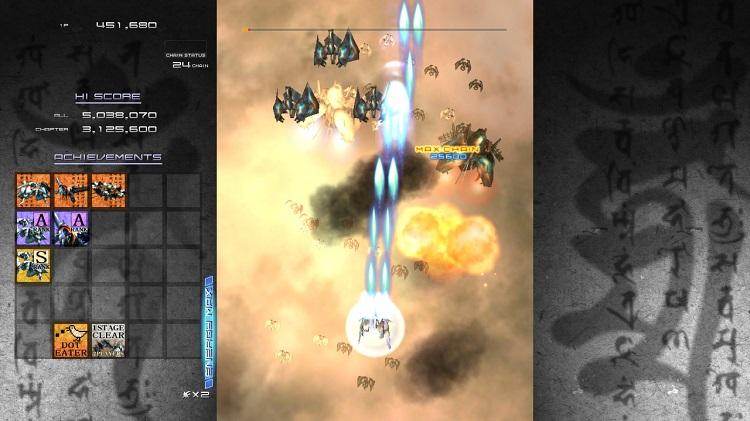
\includegraphics[width=1\textwidth]{IkaguraGameplay}
\caption{\label{fig:art}Gameplay from Ikagura(1998)}
\end{figure}
  

\begin{figure}[h!]
\centering
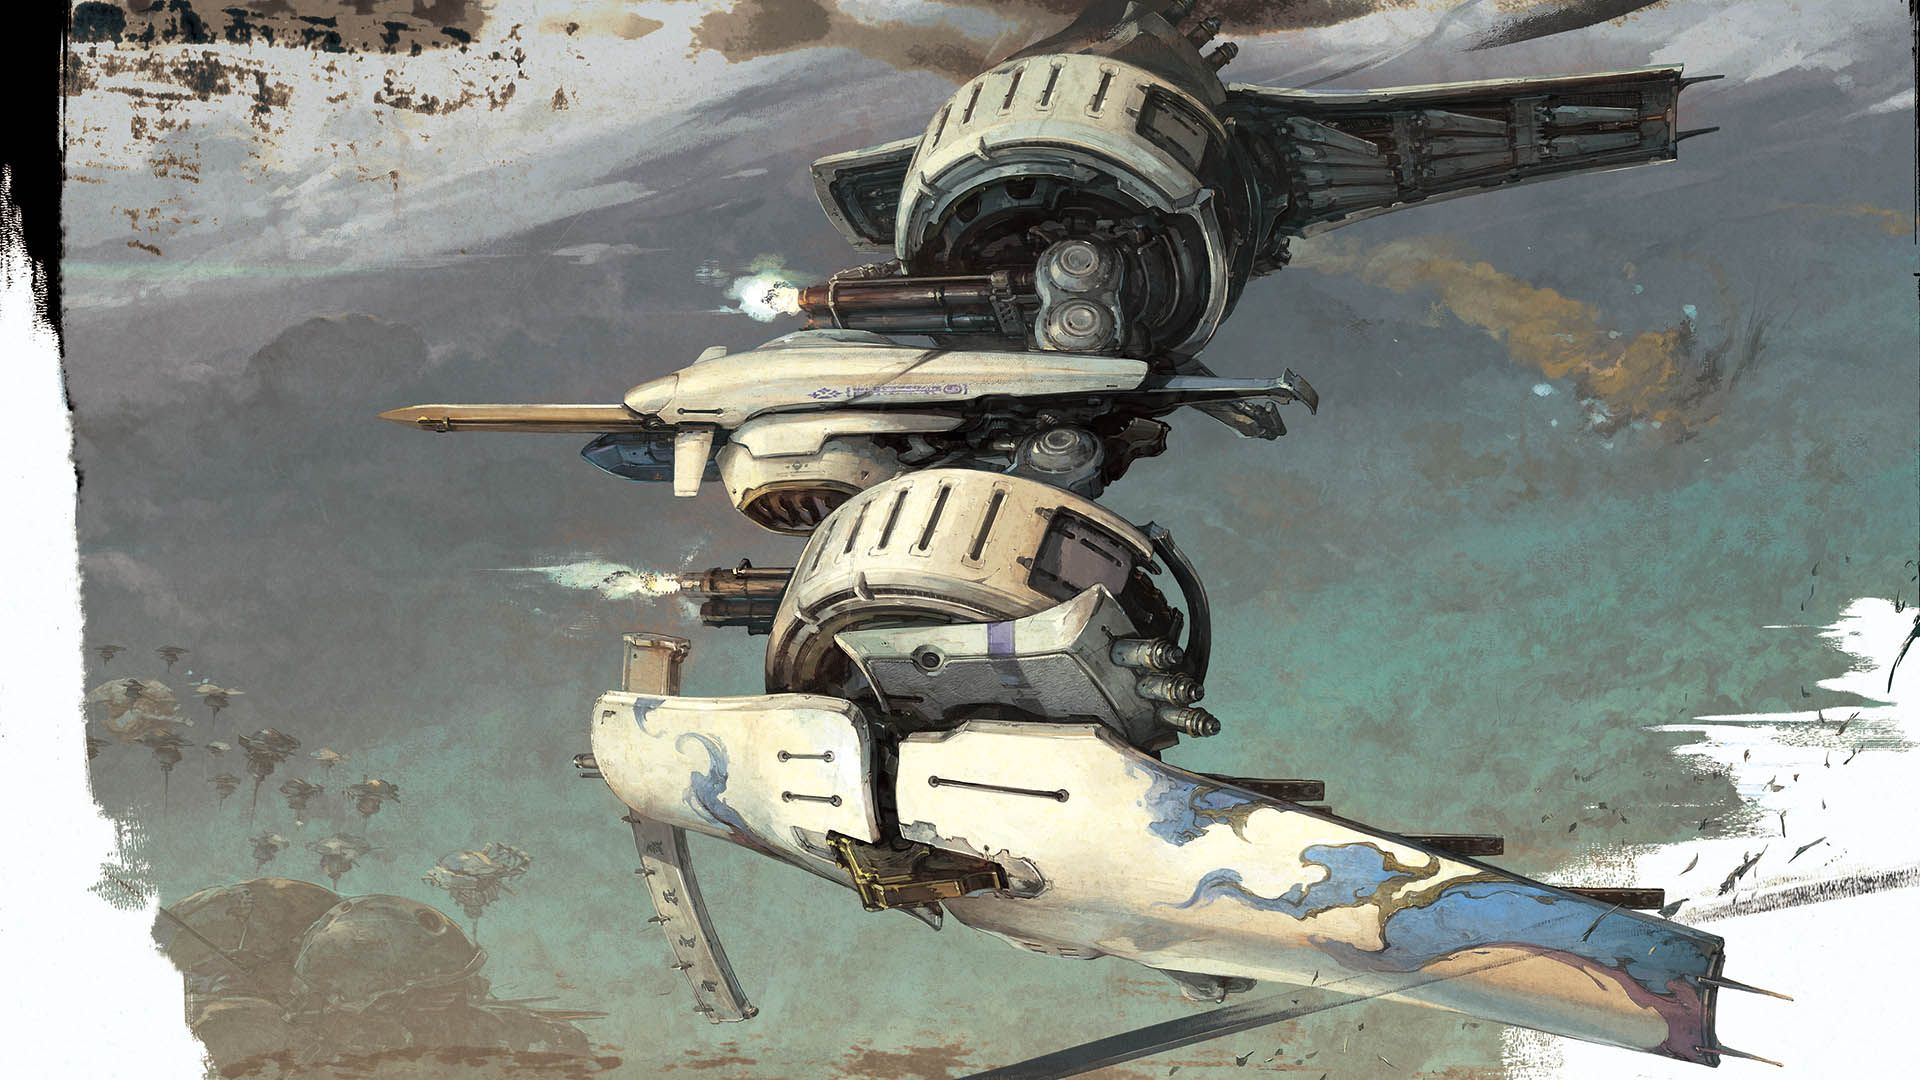
\includegraphics[width=1\textwidth]{Ikagura}
\caption{\label{fig:art}Art from Ikagura(1998)}
\end{figure}

\begin{figure}[h!]
\centering
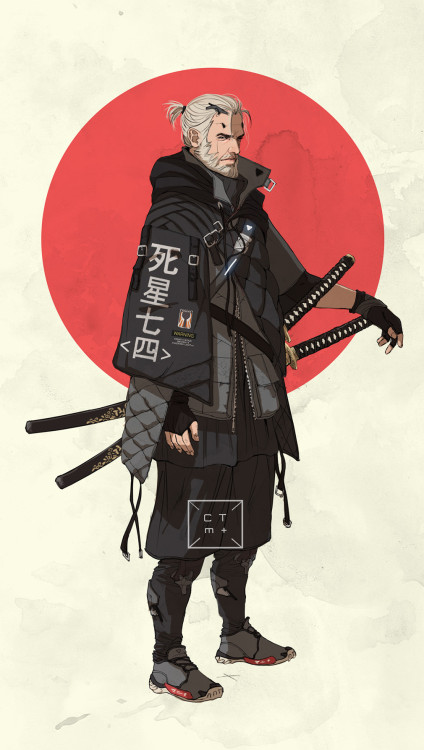
\includegraphics[width=0.5\textwidth]{Warrior}
\caption{Sci-fi warrior}
\end{figure}

\begin{figure}[h!]
\centering
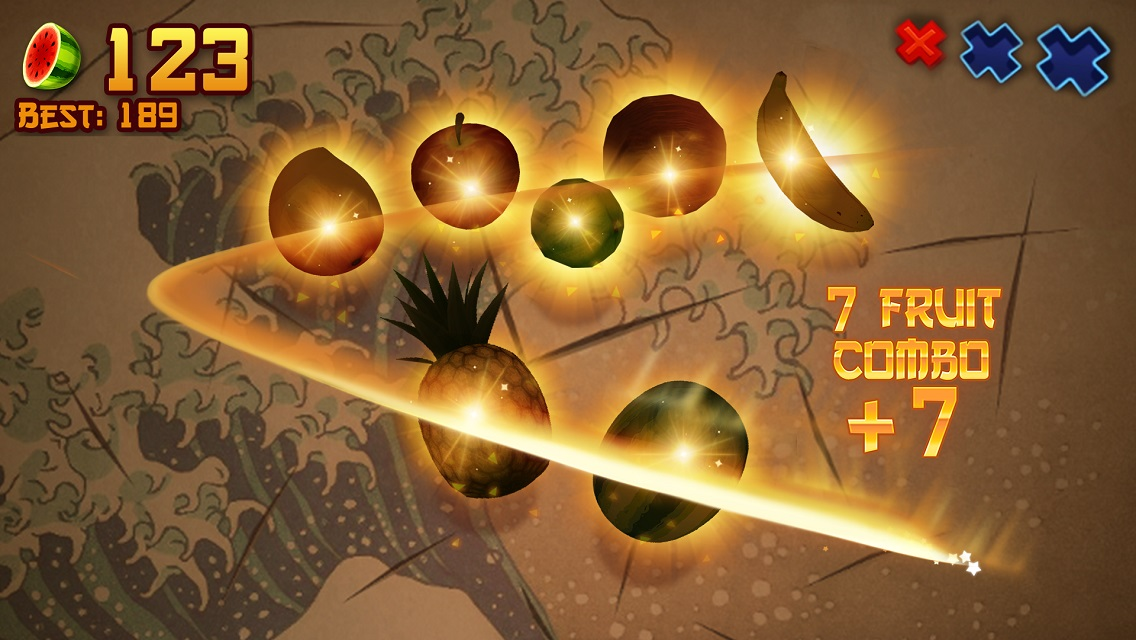
\includegraphics[width=1\textwidth]{FruitNinja}
\caption{Gameplay from 'Fruit Ninja'(2010)}
\end{figure}

\begin{figure}[h!]
\centering
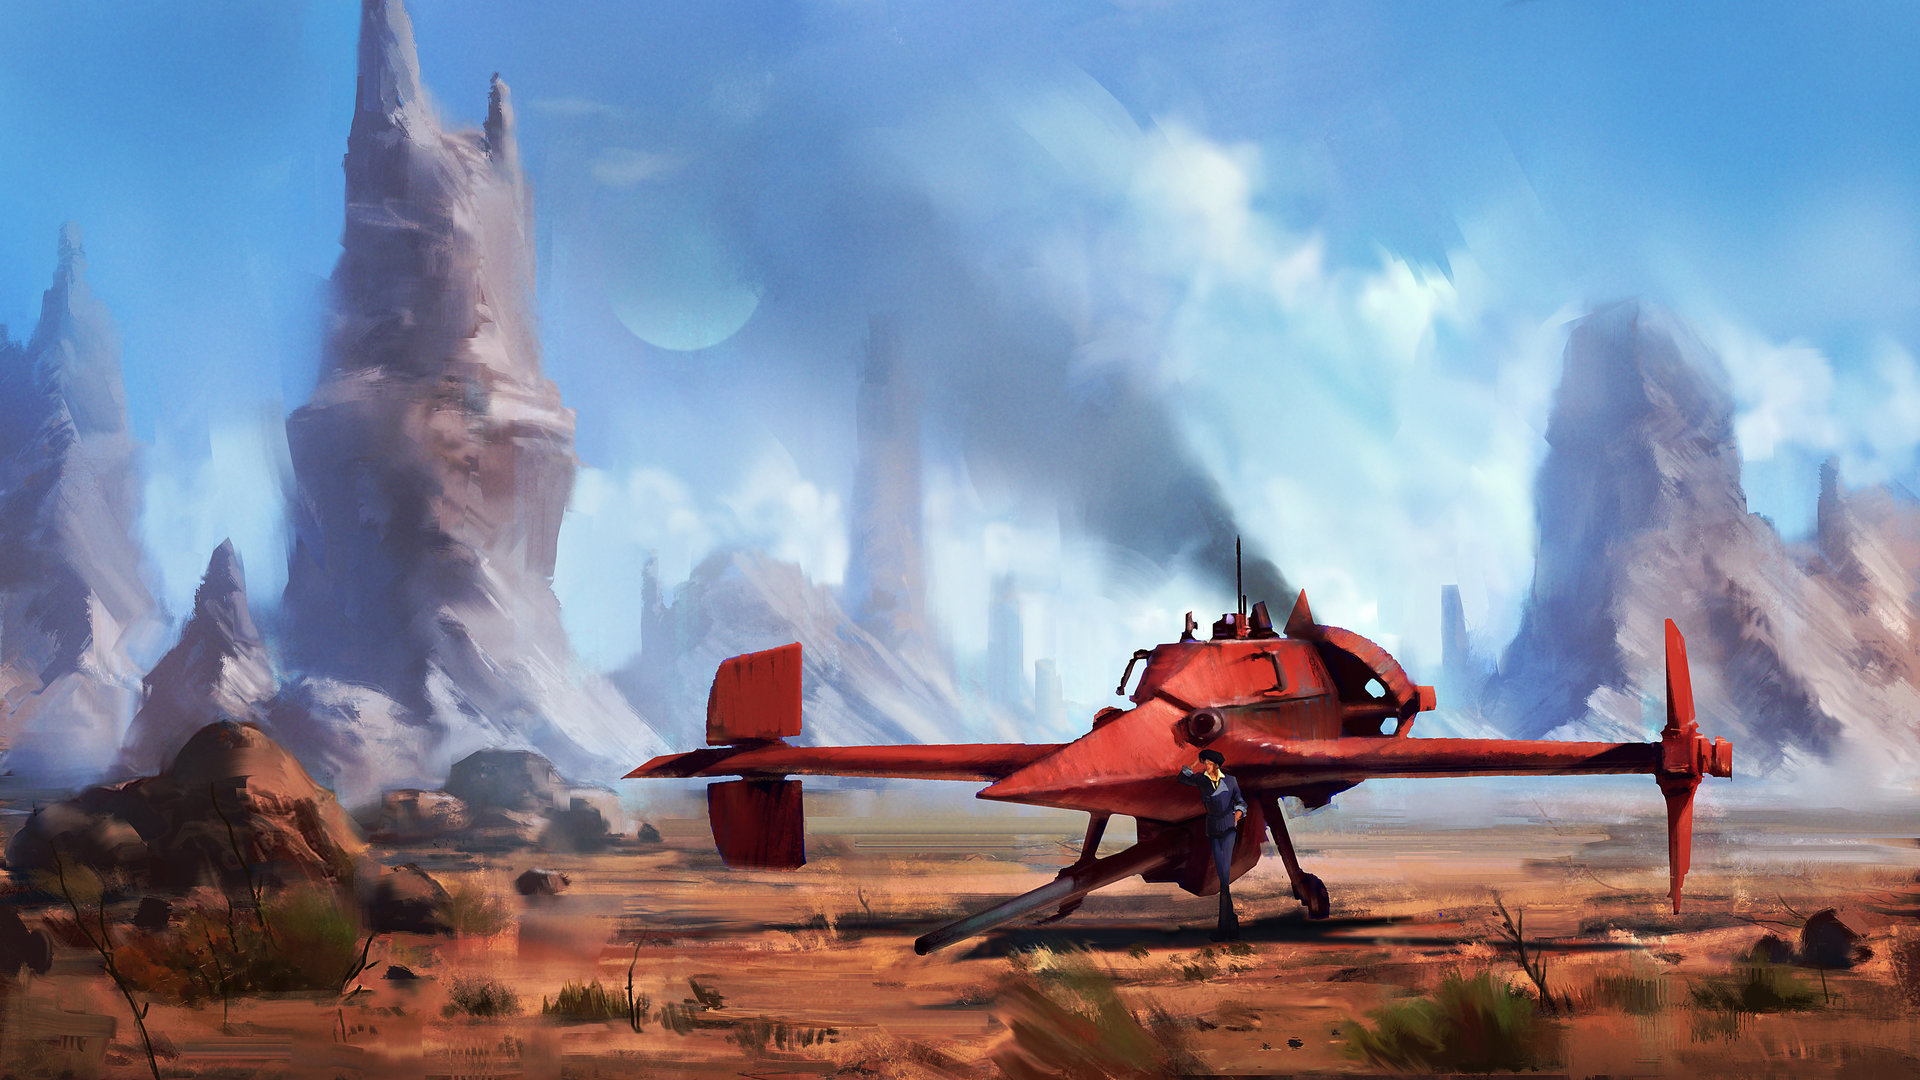
\includegraphics[width=1\textwidth]{Spaceship}
\caption{'Cowboy Bebop' concept art}
\end{figure}

\chapter{Gameplay and Game Setting}
\section{Story}
The story of the game will be kept simple to instead focus on gameplay. While exploring space in a ship called the 'Hattori', the player is teleported to an unknown location in space. The player is then confronted by horde of enemies they must defeat to survive.

\section{World/Environment}
The game will be set in space. As such, the background and enviroment may feel a bit bland, however due to the nature of the story I can expand on this and hope to make the player feel like they are making some kind of progress through space instead of feeling like a static object on a scrolling background. 

\section{User Interface}


\section{Main Objective}
The main objective of the game is to stay alive. At the end of each round/wave, the player will have a chance to rest and take count of his resources, health and current upgrades.

\section{Core Mechanics}
very important section: what are the core mechanics? be specific

\section{Controls}
describe the controls of the game 
also, add here a controller diagram if necessary 

% ______________________
% chapter Front End
% ______________________


\chapter{Front End}
description of front end such as start screen, menu screens,..  

\section{Start Screen}

\section{Menus}

\section{End Screen}

% ______________________
% chapter Game Details
% ______________________


\chapter{Technology}
This game is designed for the Universal Windows Platform but will hopefully be available in both desktop and mobile versions.

\section{Target Systems}
Android, Windows desktop and Universal Windows Platform

\section{Hardware}
Mouse and keyboard or an accelerometer/touch screen device.

\section{Development Systems/Tools}
The game will be developed in the Unity engine, using the Unity editor. C Sharp wil be the main programming language. Paint.net will be used to to design art with Visual Studio 2017 and Visual Studio code being used to write the C Sharp code. Git and GitHub are the technologies being utilized for source control. This design document was written in LaTeX and Visual Studio Code.
% ______________________
% chapter Game Details
% ______________________


\chapter{Topic and Inclusion }

describe here how you plan to address the main topic (main theme) and the 

\section{Main Theme}
\section{Inclusion}

\subsection{Diversity}
\subsection{Accessibility}
\subsection{Humanity}

% ______________________
% chapter Game Details
% ______________________

% ______________________
% chapter Game Details
% ______________________


\chapter{Timeline}

planned schedule 

\begin{table}[h]
\centering
\begin{tabular}{|l|l|l|}
\hline
Milestone & Description & Date \\\hline
& Official Start Date & 01.12.... \\
1 & Milestone Description ..  & 01.12.... \\
2 & Milestone Description ..  & 01.01.... \\
3 & Milestone Description ..  & 01.03.... \\
& End of Project & 01.04.... \\
\hline
\end{tabular}
\caption{\label{tab:schedule}Example Schedule.}
\end{table}


% ______________________
% chapter Game Details
% ______________________


\chapter{Team and Credits}

most important - who are you, who takes what role? 

e.g. :
Project Management: \\
Programming: \\ 
Art: \\ 
Design: \\ 

Additional Credits (e.g. sources of art, audio,.. ) 

%\todo[inline, color=green!40]{This is an inline comment.}

%\bibliographystyle{alpha}
%\bibliography{sample}

\end{document}